The basic idea of the HIP algorithm as it is applied to the muon
system is to fit alignables in a ``target'' tracking volume relative to a
well-aligned ``reference'' volume, usually the silicon tracker.  Muon
tracks are fitted using information from the reference volume only,
and chambers in the target are translated and rotated to minimize the
distance between muon hits and the impact points (intersections) of
tracks on the layer planes.  This differs from the conventional HIP
approach~\cite{ref:oldhip}, which iteratively aligns elements and fits tracks
in a single tracking volume.

Thick (20--60~cm) layers of iron are placed between each muon station
as a return yoke for the CMS solenoid.  In the iron, magnetic fields
are stronger than in the gas volume of the chambers, and probabilities
are higher that the muon's trajectory will 
scatter, making its direction less predictable between chambers than
within chambers.  To account for this correlation, we combine
residuals such that we obtain one independent measurement per chamber
per track.  This measurement has four components,
$\Delta x$, $\Delta y$, $\Delta \frac{dx}{dz}$, and $\Delta
\frac{dy}{dz}$, which are the differences between the propagated track's two-dimensional
location and entrance angle, respectively, with the pattern of hits in
the chamber.  We compute these four observables from a fit of the
residuals versus local $z$ to a straight line.
The reduced $\chi^2$ of the linear fit expresses
the quality of the measurement (independent of the distance between
the track and the hits), so we use $N_{\mbox{\scriptsize dof}}/\chi^2$
as a weight in the final alignment.  Station~4 DT chambers can only
measure one dimension, so they observe only $\Delta x$ and
$\Delta \frac{dx}{dz}$, and strip measurements in CSCs observe $\Delta
r\phi$ and $\Delta d(r\phi)/dz$.

The measurements described above are influenced by four categories of effects:
\begin{itemize}
\item misalignment of the target chamber (geometric residuals),
\item statistical uncertainty in the track fit,
\item propagation errors from large-angle scattering (distributes
residuals according to a power law) and the result of many small-angle
scattering events (Gaussian ``multiple scattering''),
\item biases in the track source or chamber itself.
\end{itemize}
Our goal is to identify errors of the first category, though the first
three are convoluted together in a statistical distribution, and the
fourth can only be diagnosed by an independent method (such as local
alignment techniques described in the previous sections).

Assuming that we can isolate geometric residuals ${\Delta
  x}^{\mbox{\scriptsize geom}}$, ${\Delta y}^{\mbox{\scriptsize
    geom}}$, ${\Delta \frac{dx}{dz}}^{\mbox{\scriptsize geom}}$, and
${\Delta \frac{dy}{dz}}^{\mbox{\scriptsize geom}}$, the alignment
corrections $\delta_x$, $\delta_y$, $\delta_z$, $\delta_{\phi_x}$,
$\delta_{\phi_y}$, and $\delta_{\phi_z}$ can be computed by solving
the equation:
\begin{equation}
\renewcommand{\arraystretch}{2.5}
\left(\begin{array}{c}
{\Delta x}^{\mbox{\scriptsize geom}} \\
{\Delta y}^{\mbox{\scriptsize geom}} \\
{\Delta \dfrac{dx}{dz}}^{\mbox{\scriptsize geom}} \\
{\Delta \dfrac{dy}{dz}}^{\mbox{\scriptsize geom}} \\
\end{array}\right)
=
{\renewcommand{\arraystretch}{2.5}
\left(\begin{array}{c c c c c c}
1 & 0 & -\dfrac{dx}{dz} & -y \dfrac{dx}{dz} & x \dfrac{dx}{dz} & -y \\
0 & 1 & -\dfrac{dy}{dz} & -y \dfrac{dy}{dz} & x \dfrac{dy}{dz} & x \\
0 & 0 & 0 & -\dfrac{dx}{dz} \dfrac{dy}{dz} & 1 + \left(\dfrac{dx}{dz}\right)^2 & -\dfrac{dy}{dz} \\
0 & 0 & 0 & -1 - \left(\dfrac{dy}{dz}\right)^2 & \dfrac{dx}{dz}\dfrac{dy}{dz} & \dfrac{dx}{dz}
\end{array}\right)}
\renewcommand{\arraystretch}{1.7}
\left(\begin{array}{c}
\delta_x \\
\delta_y \\
\delta_z \\
\delta_{\phi_x} \\
\delta_{\phi_y} \\
\delta_{\phi_z}
\end{array}\right) \mbox{.}
\label{eqn:dtmatrix}
\end{equation}
(The above matrix is an extension of Equation~17 in~\cite{ref:oldhip}).
For CSCs, the curvilinear residuals ${\Delta r\phi}^{\mbox{\scriptsize
geom}}$ and ${\Delta
d(r\phi)/dz}^{\mbox{\scriptsize geom}}$ introduce corrections suppressed by $r$, the radial
distance to the beamline:
\begin{equation}
\renewcommand{\arraystretch}{3}
\left(\begin{array}{c}
{\Delta r\phi}^{\mbox{\scriptsize geom}} \\
{\Delta \dfrac{dr\phi}{dz}}^{\mbox{\scriptsize geom}} \\
\end{array}\right)
=
{\renewcommand{\arraystretch}{3}
\left(\begin{array}{c c c c c c}
1 & \left[ -\dfrac{x}{r} + 3\left(\dfrac{x}{r}\right)^3 \right] & -\dfrac{dx}{dz}  & -y \dfrac{dx}{dz} & x \dfrac{dx}{dz} & -y \\
0 & -\dfrac{dx}{dz} \left(\dfrac{1}{2r}\right) & 0 & \left[ \dfrac{x}{r} - \dfrac{dx}{dz}\dfrac{dy}{dz} \right] & 1 + \left(\dfrac{dx}{dz}\right)^2 & -\dfrac{dy}{dz}
\end{array}\right)}
\renewcommand{\arraystretch}{1}
\left(\begin{array}{c}
\delta_x \\
\delta_y \\
\delta_z \\
\delta_{\phi_x} \\
\delta_{\phi_y} \\
\delta_{\phi_z}
\end{array}\right) \mbox{.}
\label{eqn:cscmatrix}
\end{equation}

To extract geometric residuals from the measurements, we construct an
ansatz describing all effects and fit it to the data.  Each of the
four observables is represented by a convolution of a Gaussian and a
Lorentzian (to model the power-law scattering tails),
\begin{equation}
f(t; \, t_0, \, \sigma, \, \gamma) = \int_{-\infty}^\infty
\frac{1}{\pi}\frac{\gamma}{(t - s - t_0)^2 + (\gamma)^2} \times 
\frac{1}{\sqrt{2\pi} \sigma} \exp\left(\frac{-s^2}{2
  \sigma^2}\right) \, ds \mbox{.}
\label{eqn:fitfunction}
\end{equation}
Position residuals are correlated with their corresponding angle
residuals because any error in the propagated track's direction
upstream of the chamber causes errors in its position to grow.
Therefore, a 2-D distribution of $\Delta x$ and $\Delta \frac{dx}{dz}$
is skewed by a parameter $\alpha_{\Delta x}$.  A fit function for all
four residuals, $F$, is the product of four instances of $f$:
\begin{multline}
F\bigg(\Delta x, \Delta y, \Delta \tfrac{dx}{dz}, \Delta \tfrac{dy}{dz}; \\
{\Delta x}_0, {\Delta y}_0, {\Delta \frac{dx}{dz}}_0, {\Delta \frac{dy}{dz}}_0,
\sigma_{\Delta x}, \sigma_{\Delta y}, \sigma_{\Delta \tfrac{dx}{dz}}, \sigma_{\Delta \tfrac{dy}{dz}}, 
\gamma_{\Delta x}, \gamma_{\Delta y}, \gamma_{\Delta \tfrac{dx}{dz}}, \gamma_{\Delta \tfrac{dy}{dz}}, 
\alpha_{\Delta x}, \alpha_{\Delta y}) = \\
f\bigg(\Delta x; \, \big({\Delta x}_0 + \alpha_{\Delta x} \Delta \tfrac{dx}{dz}\big), \, \sigma_{\Delta x}, \, \gamma_{\Delta x}\bigg) \, \times \,
f\bigg(\Delta \tfrac{dx}{dz}; \, {\Delta \tfrac{dx}{dz}}_0, \, \sigma_{\Delta \tfrac{dx}{dz}}, \, \gamma_{\Delta \tfrac{dx}{dz}}\bigg) \\
f\bigg(\Delta y; \, \big({\Delta y}_0 + \alpha_{\Delta y} \Delta \tfrac{dy}{dz}\big), \, \sigma_{\Delta y}, \, \gamma_{\Delta y}\bigg) \, \times \,
f\bigg(\Delta \tfrac{dy}{dz}; \, {\Delta \tfrac{dy}{dz}}_0, \, \sigma_{\Delta \tfrac{dy}{dz}}, \, \gamma_{\Delta \tfrac{dy}{dz}}\bigg)
\end{multline}

The peak of this distribution, $({\Delta x}_0, \, {\Delta y}_0,
\, {\Delta \frac{dx}{dz}}_0, \, {\Delta\frac{dy}{dz}}_0)$, can be
identified as the geometric residuals on the left-hand-side of
Equation~\ref{eqn:dtmatrix} because the observed distribution of
residuals is further convoluted by misalignment.  The effect of
misalignment is not random; its distribution would be described by a
system of delta distributions that simply replace $({\Delta x}_0, \, {\Delta y}_0,
\, {\Delta \frac{dx}{dz}}_0, \, {\Delta\frac{dy}{dz}}_0)$ with 
$({\Delta x}^{\mbox{\scriptsize geom}},\mbox{ }{\Delta
y}^{\mbox{\scriptsize geom}},\mbox{
}{\Delta \frac{dx}{dz}}^{\mbox{\scriptsize geom}},\mbox{
}{\Delta \frac{dy}{dz}}^{\mbox{\scriptsize geom}})$ and introduce a
dependence on the track impact positions $x$, $y$ and entrance angles
$\tfrac{dx}{dz}$, $\tfrac{dy}{dz}$.  The final fit function has 16
parameters and 8 dimensions for DT stations 1--3, 11 parameters and 6
dimensions for CSCs, and 10 parameters, 6 dimensions for DT station~4
(no access to $\delta_y$).  The most relevant projections of an
example fit are shown in Figure~\ref{fig:examplefit}.  The fit is
performed by MINUIT~\cite{ref:minuit} with an unbinned maximum
likelihood method, using the weights described above.

\begin{figure}
\begin{center}
\subfigure[Projection of residuals onto impact point and entrance angle, before alignment.]{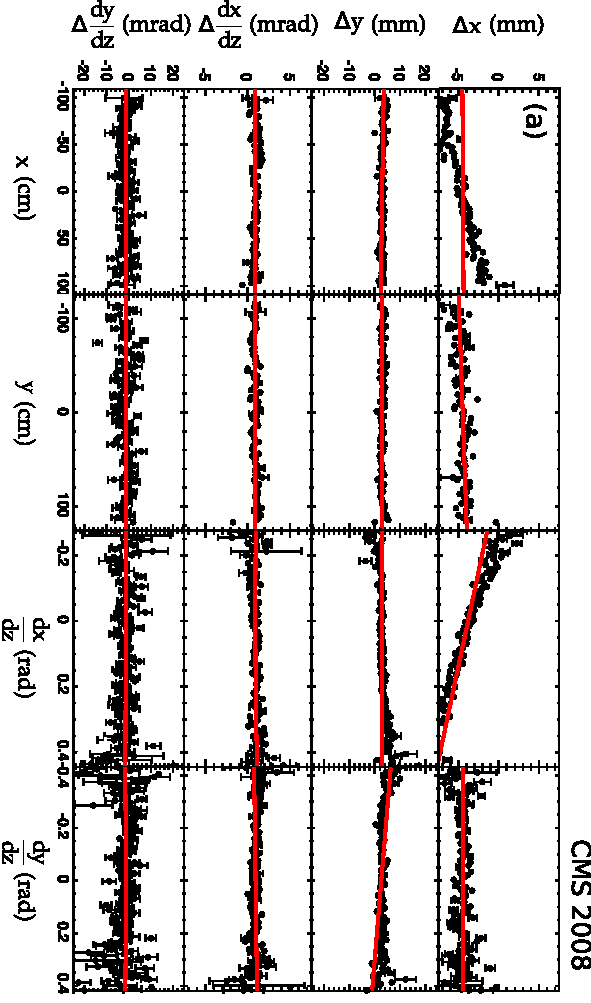
\includegraphics[height=\linewidth, angle=90]{plots/gma_hip_algorithm/exampleData_wh0st1sec10_polybefore.pdf}}

\subfigure[Projection of residuals onto impact point and entrance angle, after alignment. \label{fig:examplefitb}]{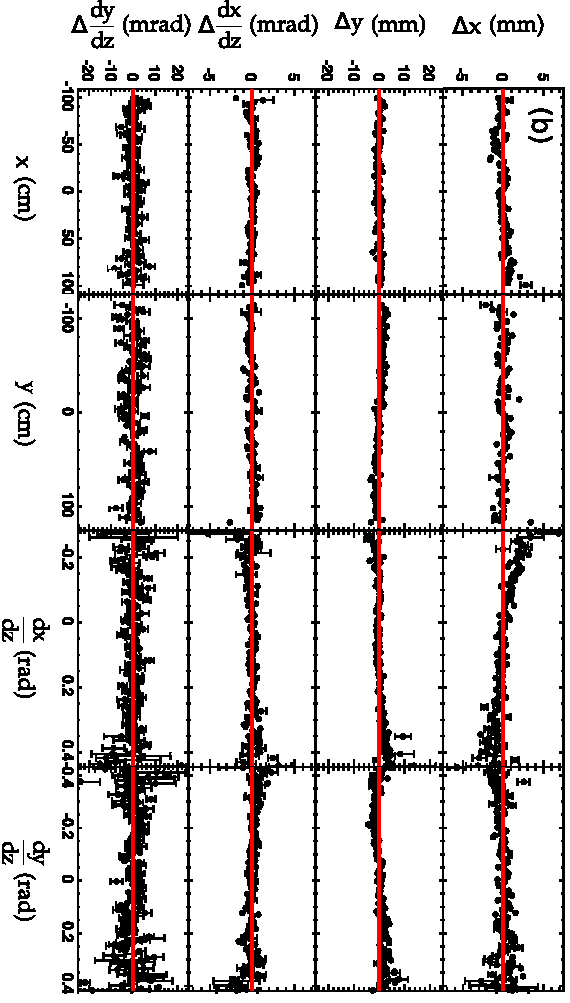
\includegraphics[height=\linewidth, angle=90]{plots/gma_hip_algorithm/exampleData_wh0st1sec10_polyafter.pdf}}
\end{center}

\caption{An example fit to cosmic ray data (DT wheel~0, station~1, sector~10) from the HIP algorithm.  The red lines are projections of the fit result. \label{fig:examplefit}}
\end{figure}

If the magnetic field or material maps are not perfectly represented
in track propagation, residuals will be biased as an antisymmetric
function of track curvature, $q/p_T$.  To correct for any such errors,
we split the sample into two bins, one for each charge $q$, and
perform the alignment separately in each bin.  Muons and antimuons
have the same spectral distribution in cosmic rays (though not the
same flux), so a simple average of the $q<0$ and $q>0$ results cancels the
antisymmetric bias in all alignment corrections except $\delta_z$.
The difference of the two bins is maximally sensitive to the bias and
can be used to measure it.

Repeated applications of the procedure converge quickly to an optimal
solution.  Significant corrections are only observed in the first and
second iterations (in data and simulation), so we always perform three
iterations.
